\documentclass{article}
\usepackage{graphicx}
\usepackage{amsmath}
\usepackage{amsfonts}
\usepackage{bookmark}
\usepackage{booktabs}
\usepackage{exercises}
\graphicspath{ {./images/8.2} }
\usepackage{indentfirst}
\usepackage{amsthm}
\usepackage{yhmath}
\usepackage{geometry}
\usepackage{placeins}
\usepackage{csquotes}
\usepackage{pgfplots}
\newcommand*{\oldneg}{\mathord{\sim}}
\newcommand\showdiv[1]{\overline{\smash{)}#1}}
\newcommand\Mydiv[1]{%
\smash{\raise.3ex\hbox{$\big)$}}\mkern-8mu
        \overline{\enspace\strut#1}}
\setlength{\tabcolsep}{5pt}
\theoremstyle{definition}
\newtheorem{definition}{Definition}

\setlength{\parindent}{.5in}
\setlength{\parskip}{12pt}
\renewcommand{\arraystretch}{2}
\geometry{margin=1in}
\newcommand{\?}{\stackrel{?}{=}}
\pgfplotsset{width=7cm,compat=1.18}\usepgfplotslibrary{statistics}

\title{8.2 Answers}
\begin{document}
\maketitle

\section*{1}
A parabola is the set of all points in a plane equidistant from a point called the focus and a line called the directrix.

\section*{2}
The graph of $x^2=4py$ has a focus at $(0,p)$, a directrix of $y=-p$, and its axis of symmetry is the line $x=0$. In contrast, the graph of 
$y^2=4px$ has a focus at $(p,0)$, a directrix of $x=-p$, and its axis of symmetry is the line $y=0$. 

\section*{19}
\begin{samepage}
We are given the equation \[ \frac{1}{8}x^2-y=0 \] \[ x^2=8y \] Thus $p=\frac{8}{4}=2$, meaning, because $p>0$, the focus is $(0,2)$, the directrix is $y=-2$, and the axis of symmetry is 
$x=0$:\newline
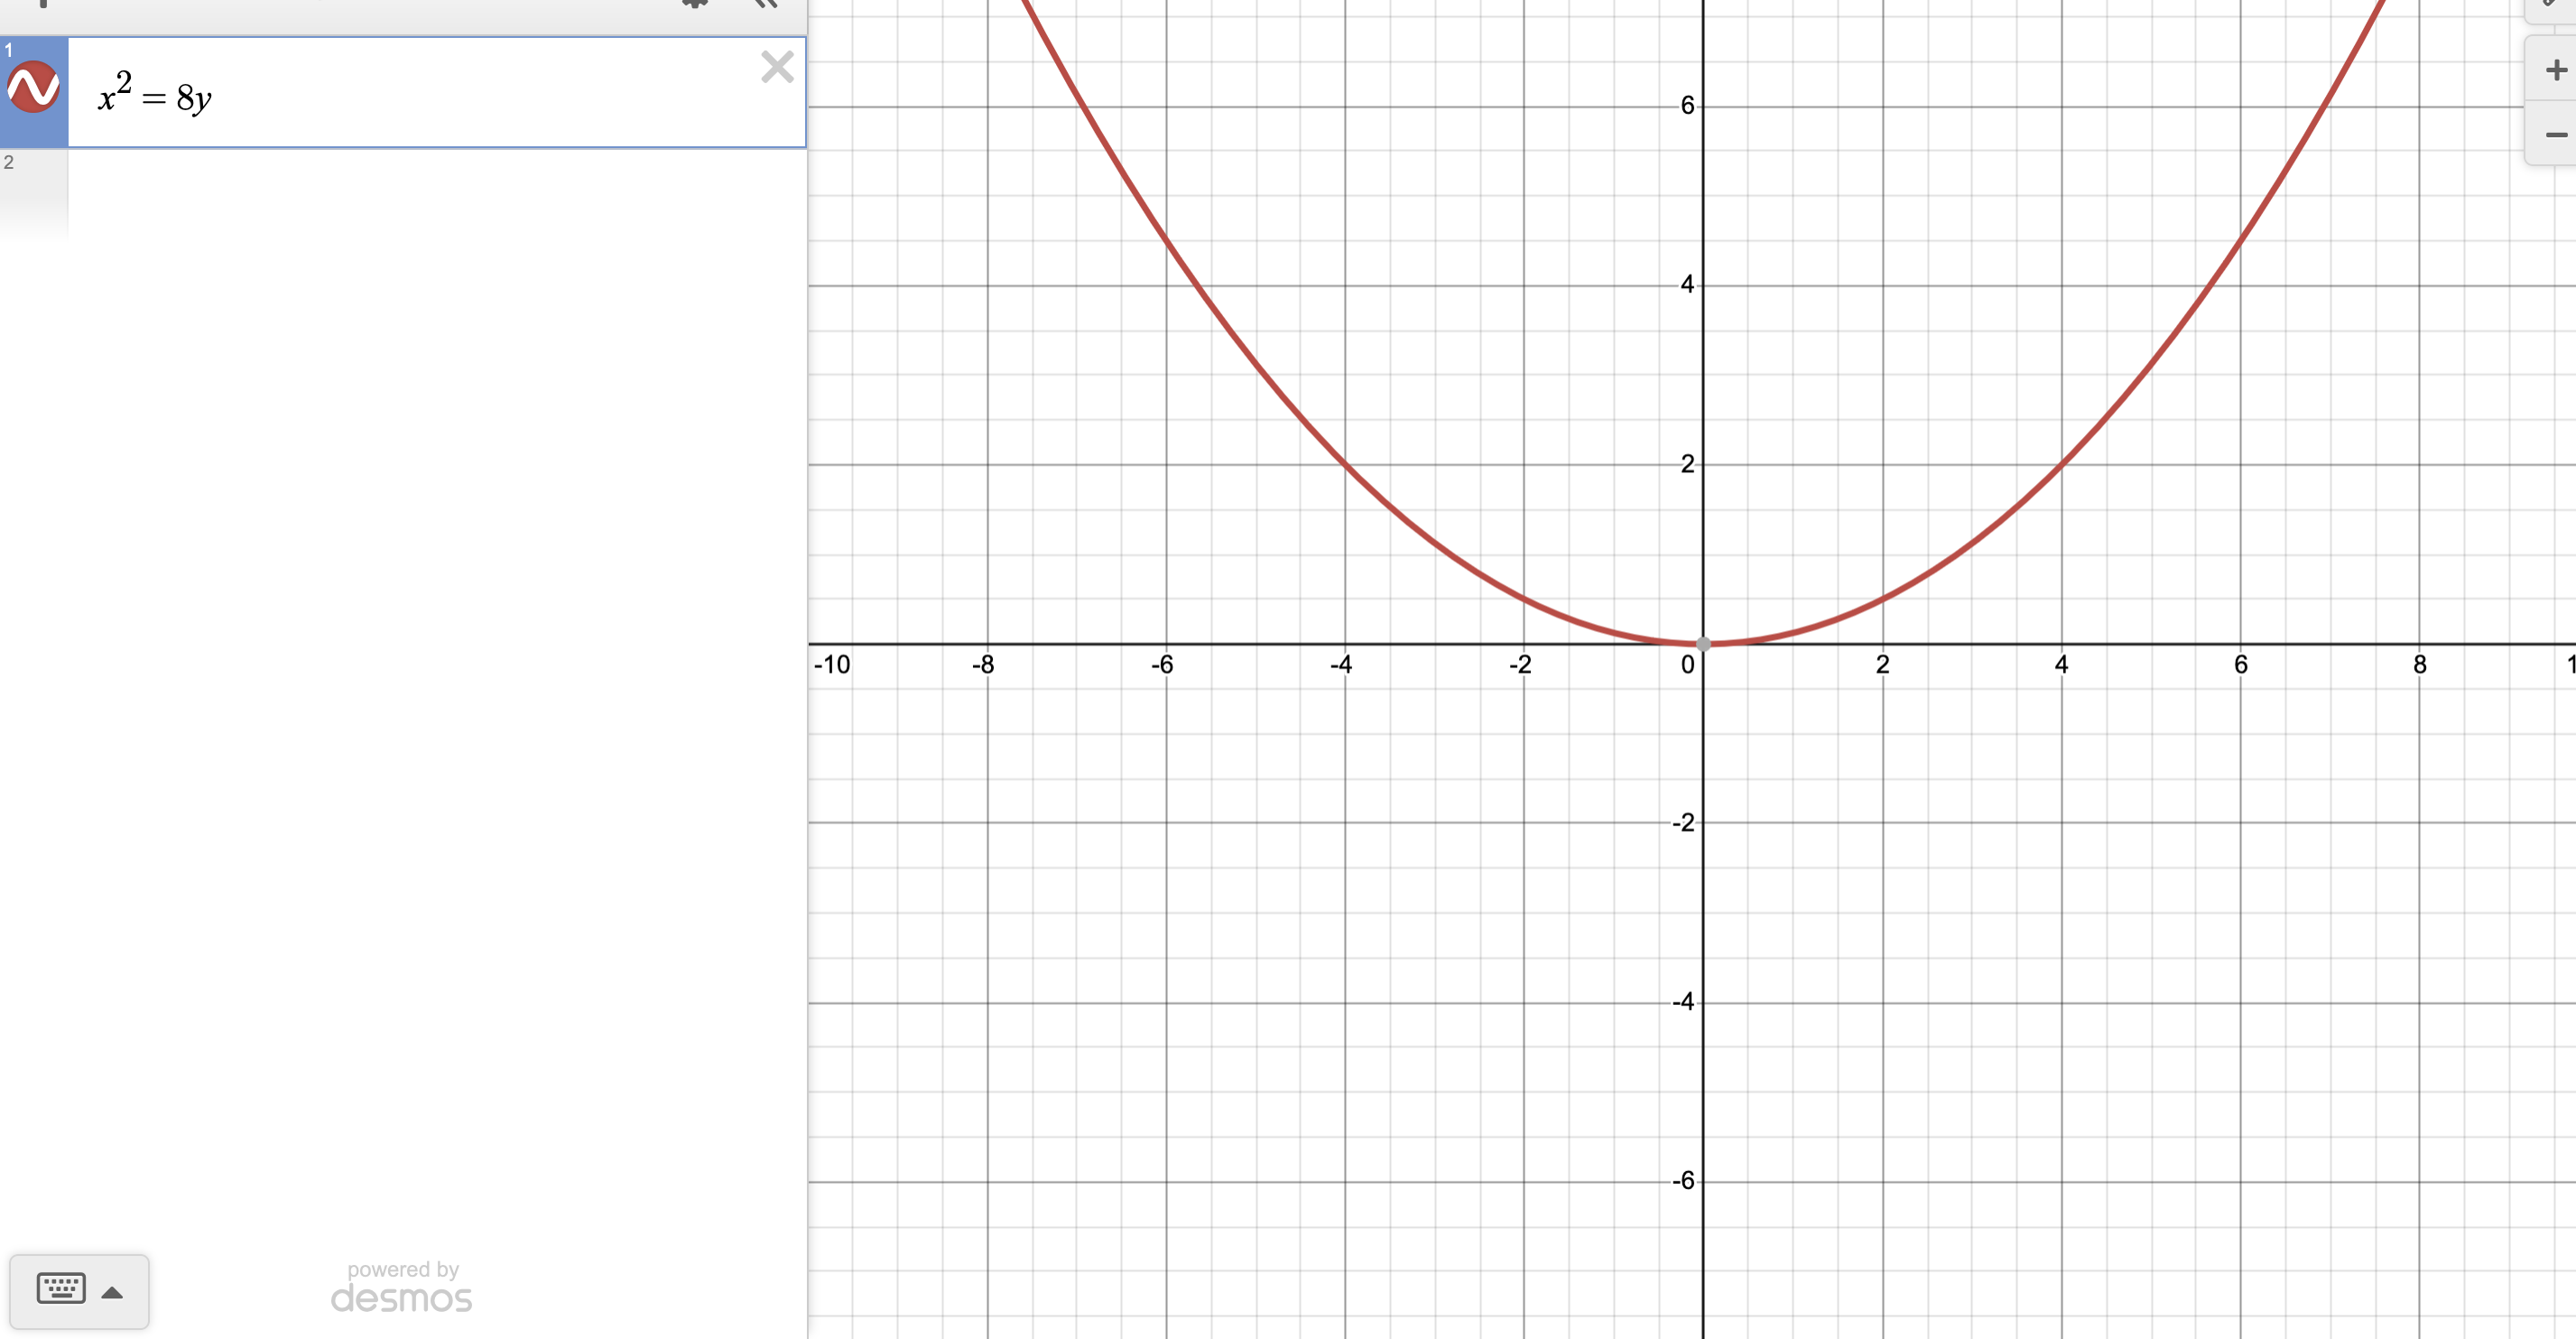
\includegraphics[width = 4in, height = 4in]{19}
\end{samepage}

\section*{20}
\begin{samepage}
We are given the equation \[ 4x-11y^2=0 \] \[ y^2=\frac{4}{11}x \] Thus $p=\dfrac{\frac{4}{11}}{4}=\frac{1}{11}$, meaning the focus is $(\frac{1}{11},0)$, the directrix is 
$x=-\frac{1}{11}$, and the axis of symmetry is $y=0$:\newline
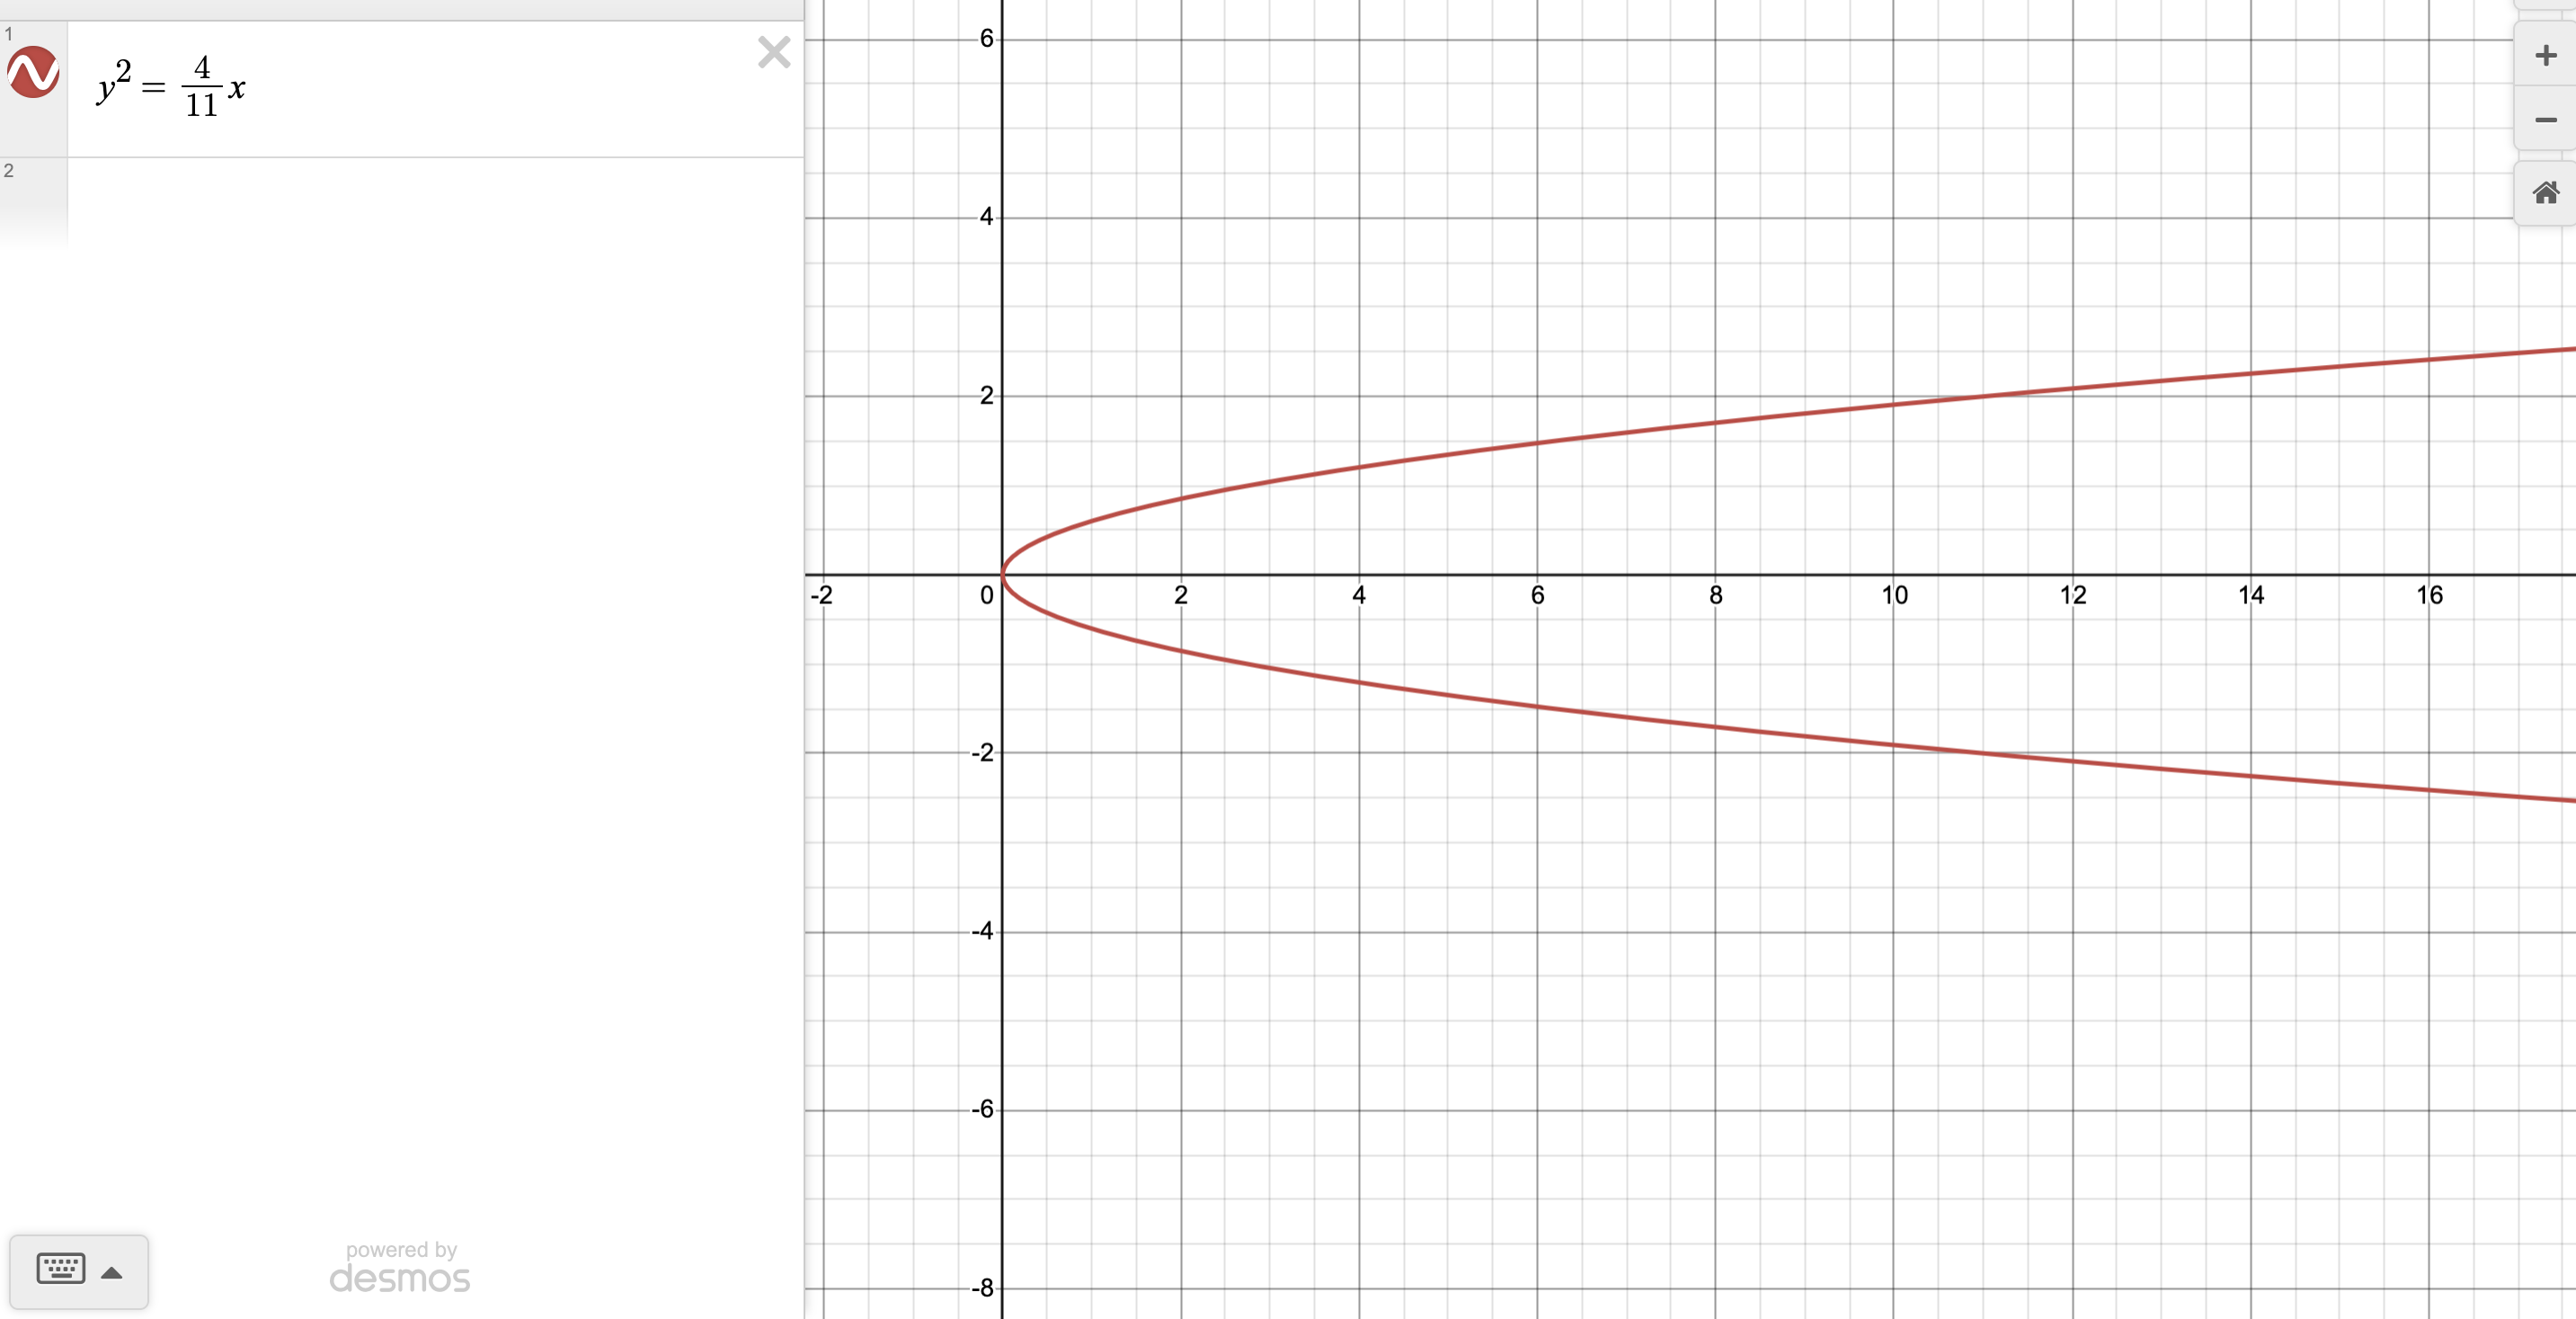
\includegraphics[width = 4in, height = 4in]{20}
\end{samepage}

\section*{21}
\begin{samepage}
We are given the equation \[ 5x^2+12y=0 \] \[ x^2=-\frac{12}{5}y \] Thus $p=\dfrac{-\frac{12}{5}}{4}=-\frac{3}{5}$, meaning the focus is $(0,-\frac{3}{5})$, the directrix is
$y=\frac{3}{5}$, and the axis of symmetry is $x=0$:\newline
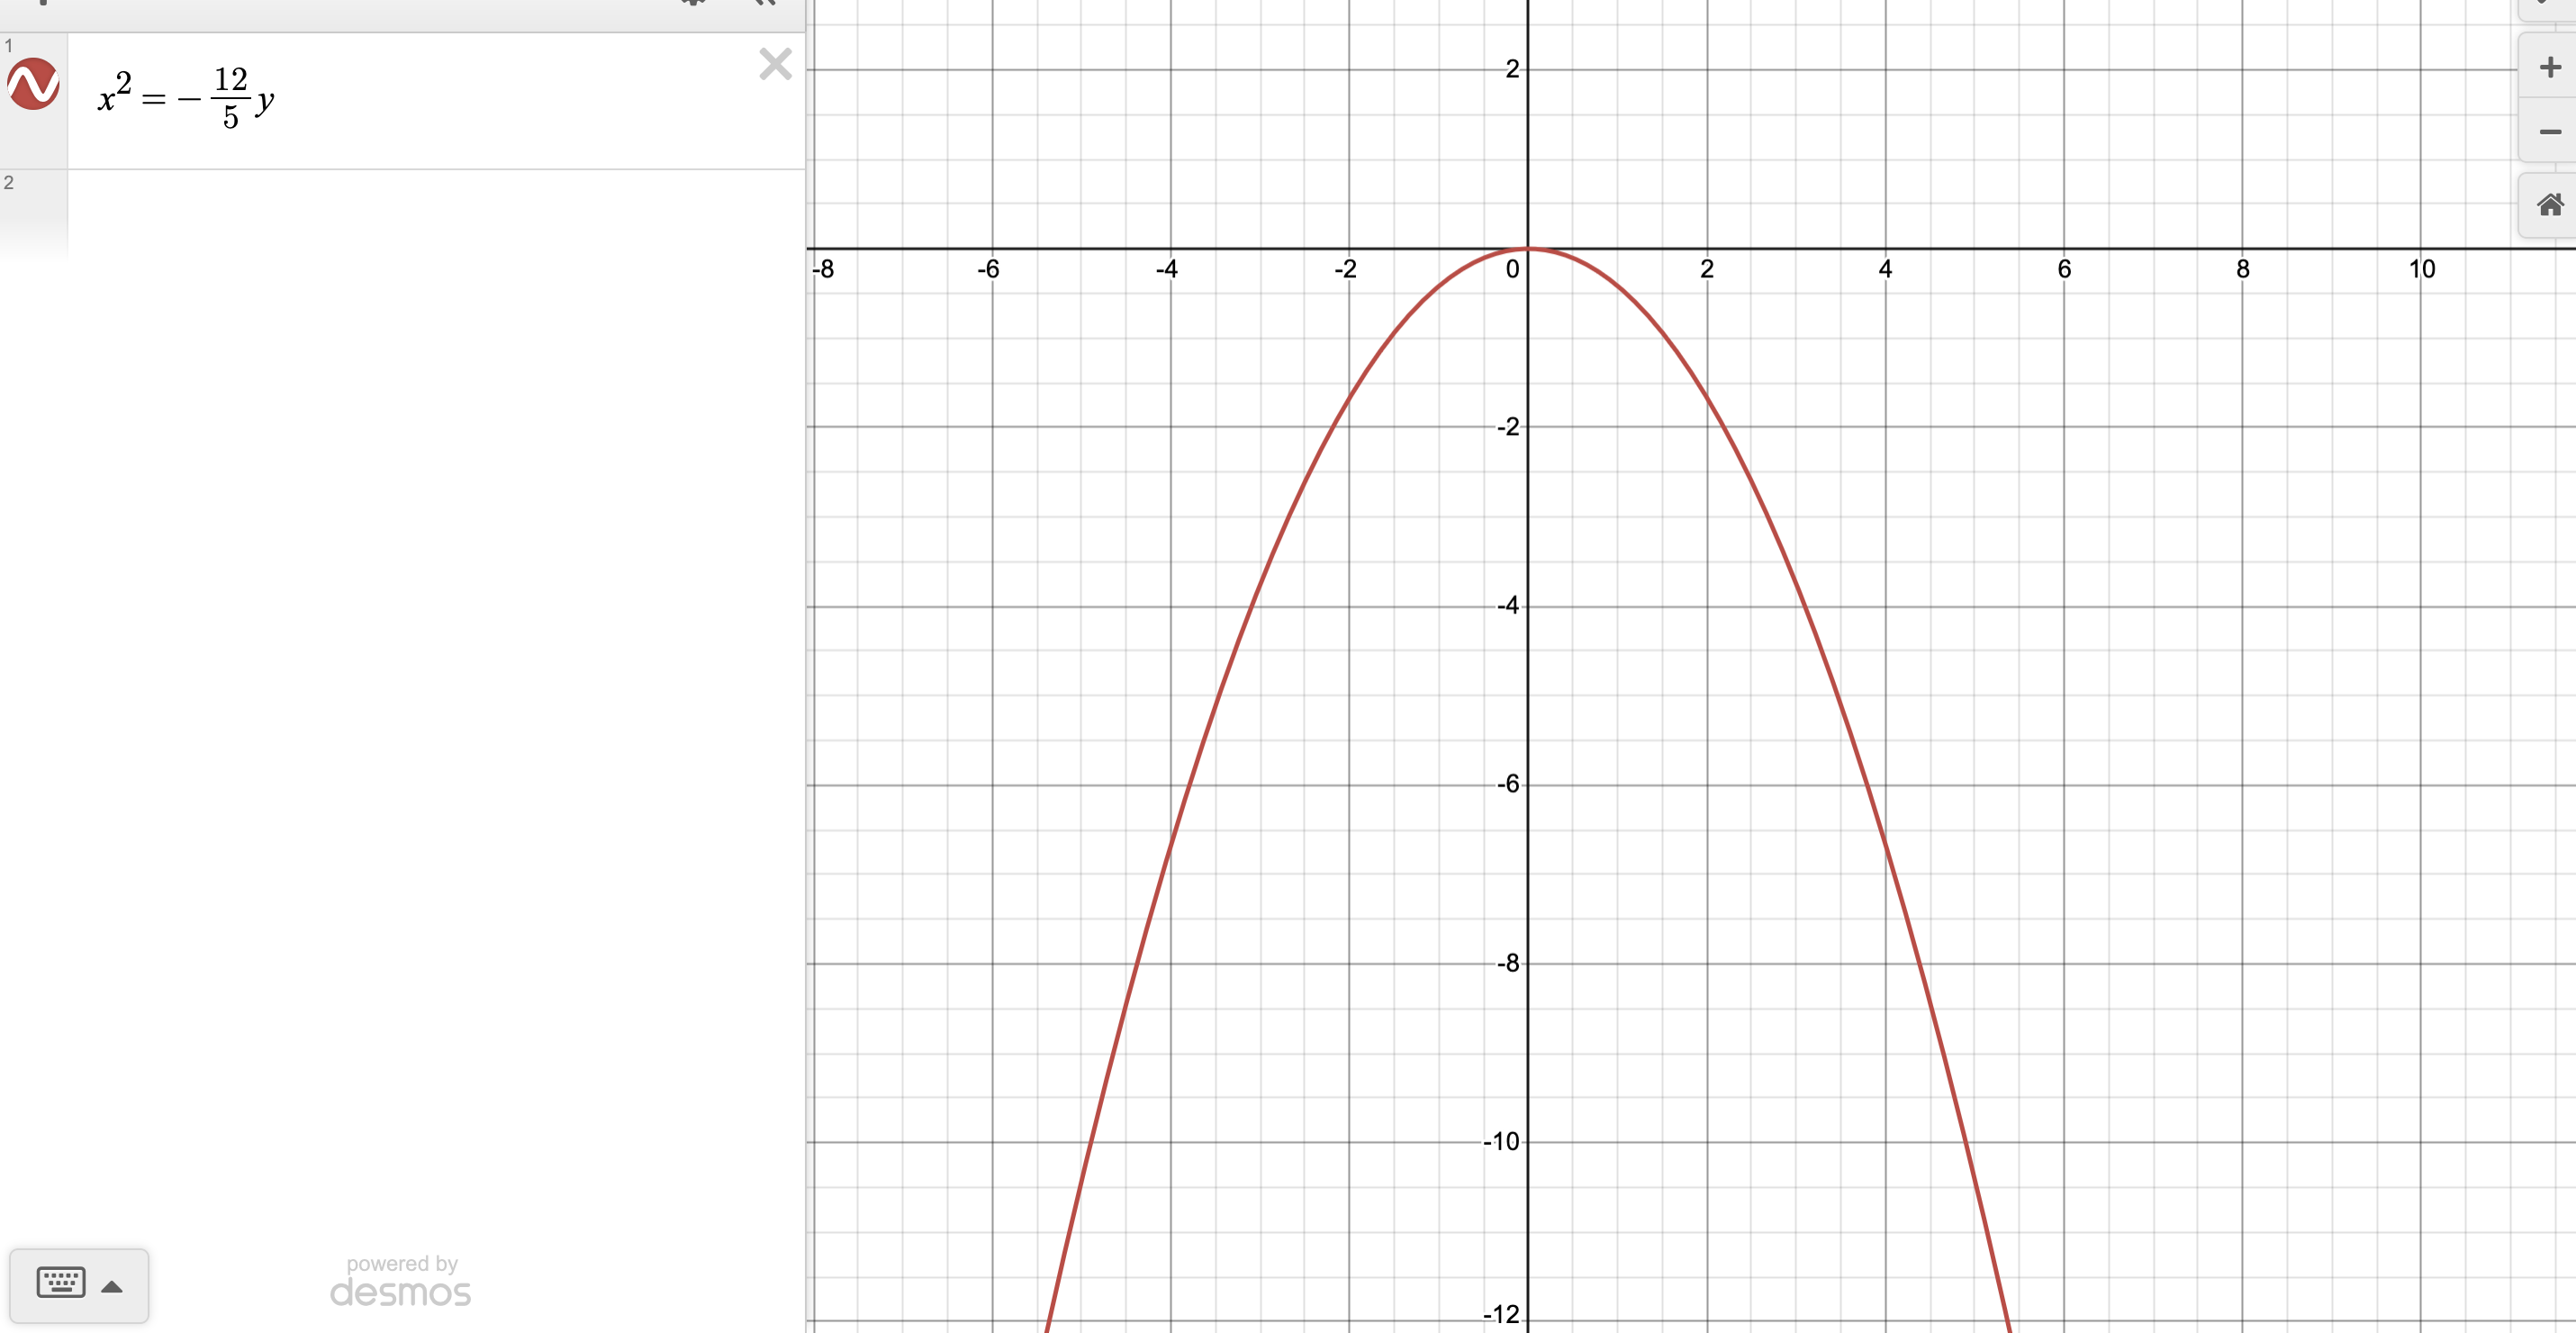
\includegraphics[width = 4in, height = 4in]{21}
\end{samepage}

\section*{22}
\begin{samepage}
We are given the equation \[ -5x+\frac{1}{3}y^2=0 \] \[ y^2=15x \] Thus $p=\frac{15}{4}$, meaning the focus is $(\frac{15}{4},0)$, the directrix is $x=-\frac{15}{4}$, and the 
axis of symmetry is $y=0$:\newline
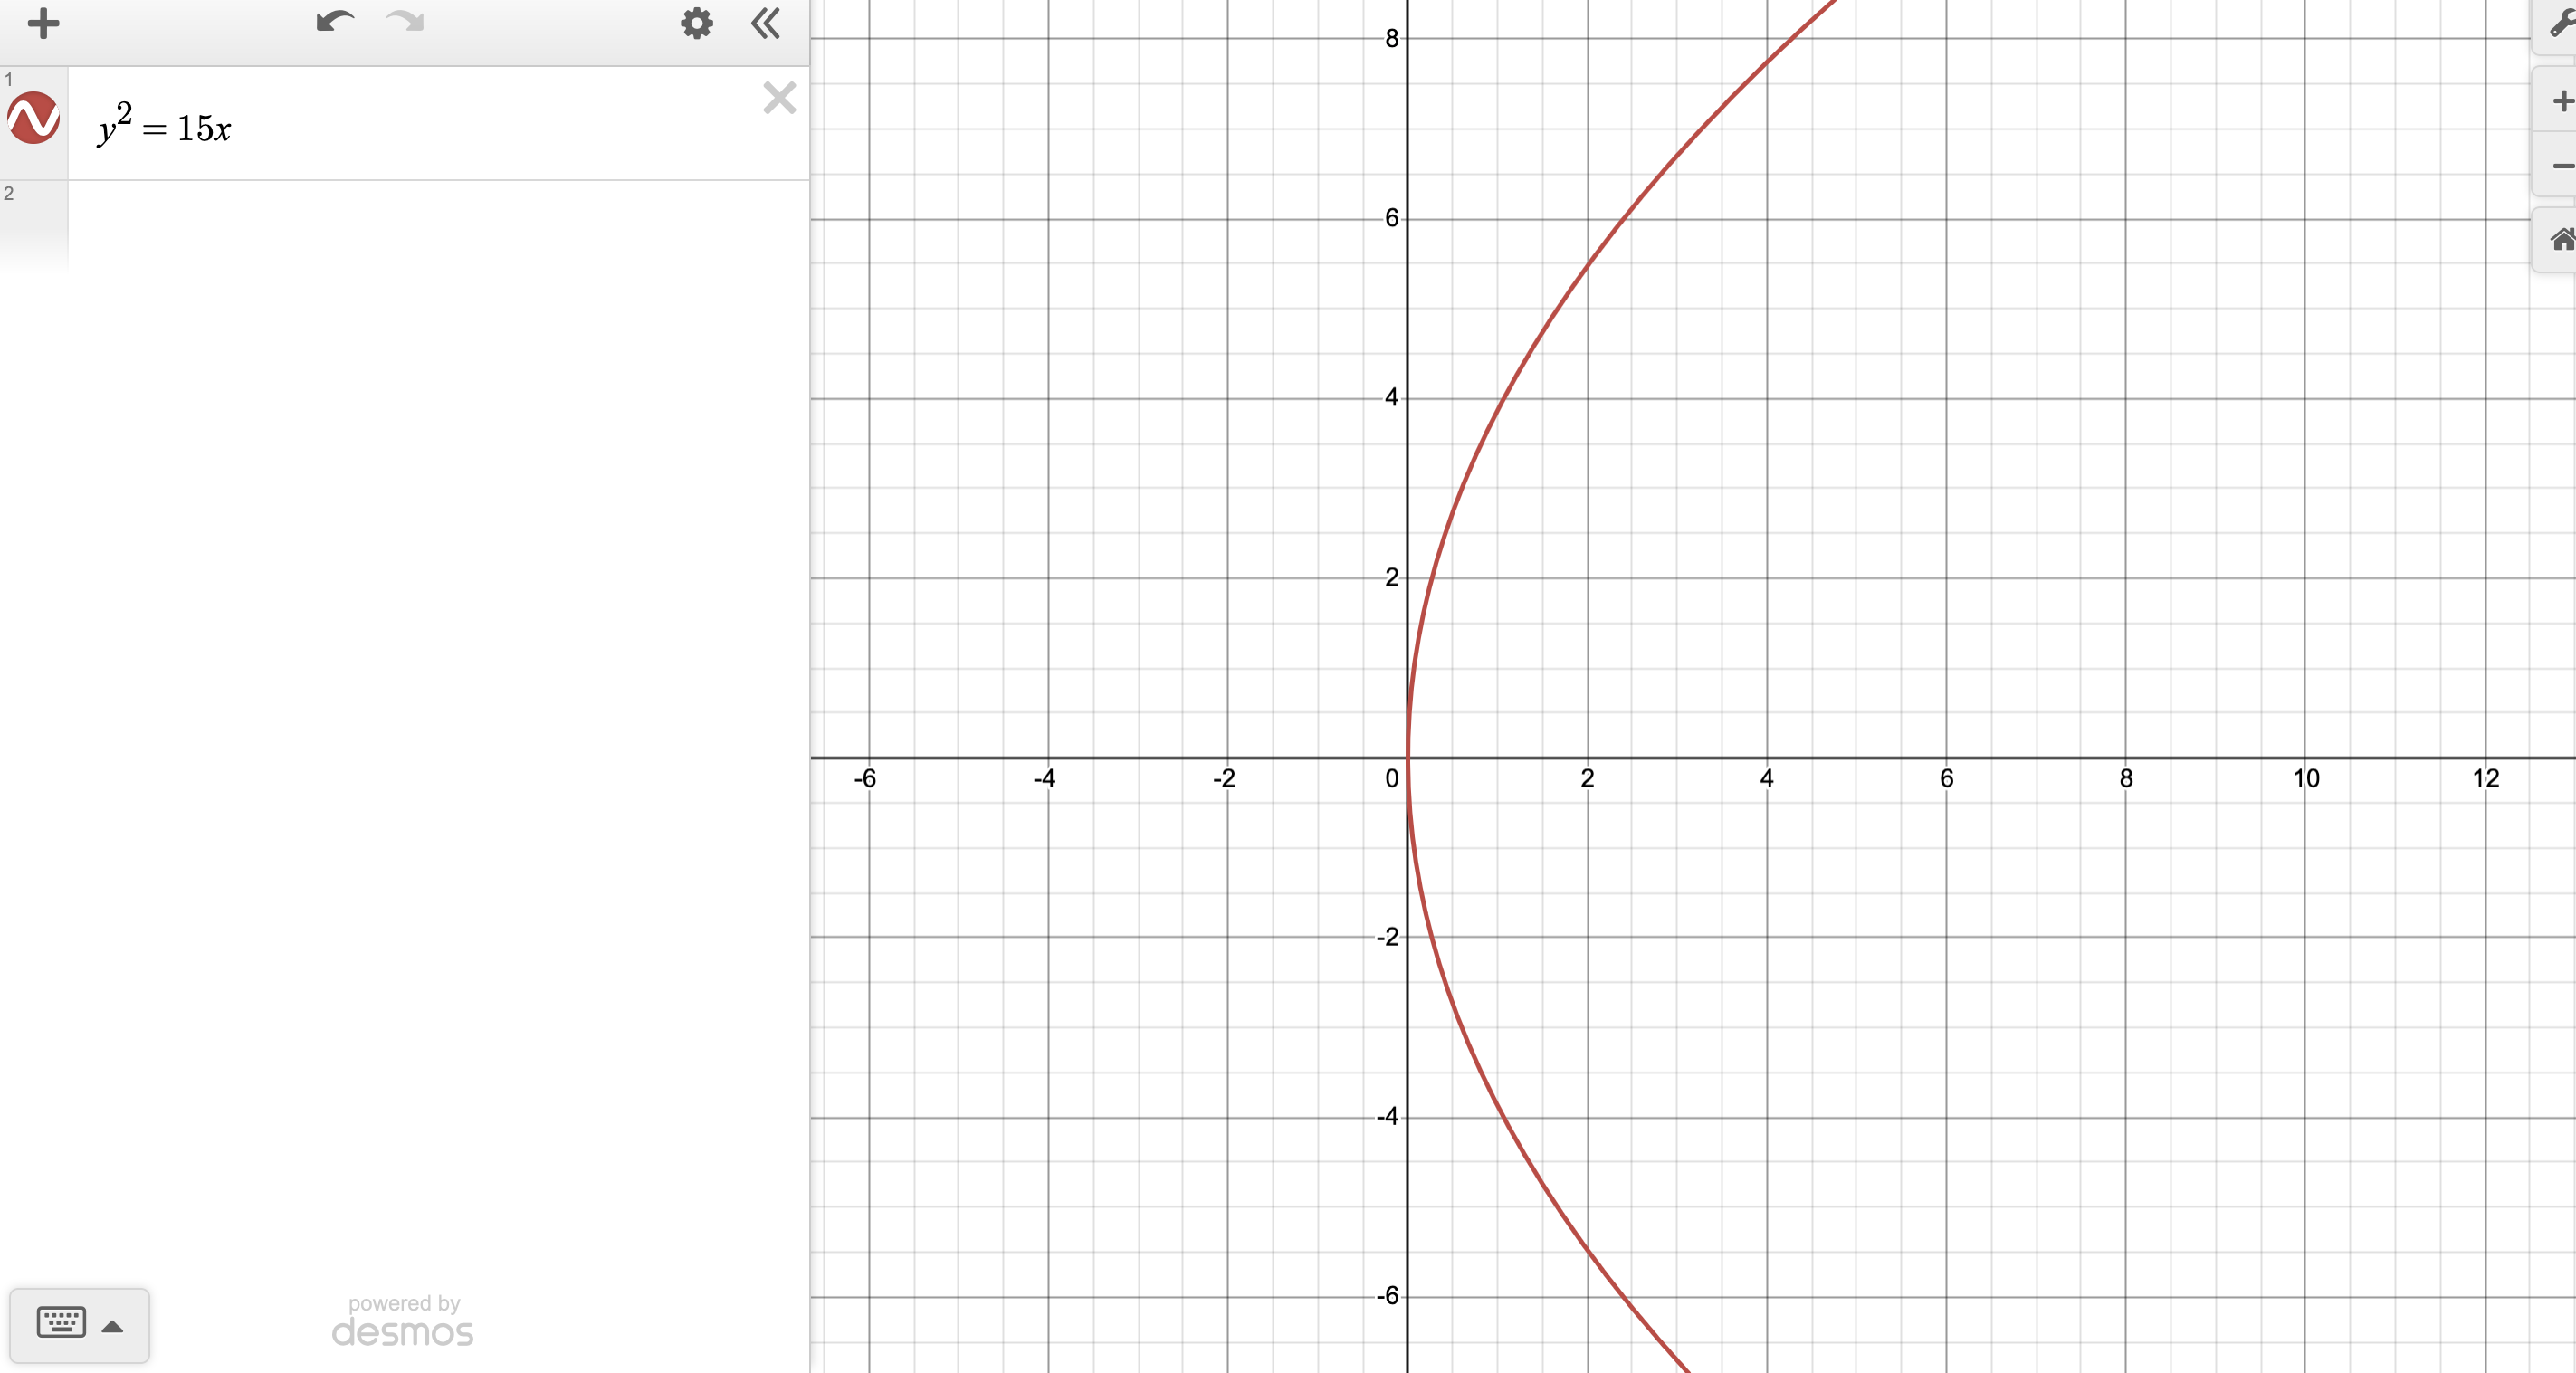
\includegraphics[width = 4in, height = 4in]{22}
\end{samepage}

\section*{25}
We are given \[ 15y+3x^2=0 \] \[ x^2=-5y \] Thus $p=-\frac{5}{4}=-1.25$ and the directrix is $y=1.25$. D

\section*{35}
We are given a focus of $(0,-\frac{3}{8})$. Thus the equation is of the form $x^2=4py$, in particular, 
$x^2=4(-\frac{3}{8})y=-\frac{3}{2}y$.

\section*{36}
We are given a focus of $(\frac{5}{2},0)$. Thus the equation is of the form $y^2=4px$, in particular,
$y^2=4(\frac{5}{2})x=10x$.

\section*{37}
We are given a focus of $(-\frac{9}{16},0)$. Thus the equation is of the form $y^2=4px$, in particular,
$y^2=4(-\frac{9}{16})x=-\frac{9}{4}x$. 

\section*{38}
We are given a focus of $(-8,0)$. Thus the equation is of the form $y^2=4px$, in particular,
$y^2=4(-8)x=-32x$. A

\section*{49}
We are given a directrix of $y=-\frac{11}{6}$. We then know that the equation is of the form $x^2=4py$, and 
$p=-(-\frac{11}{6})=\frac{11}{6}$ and thus the equation is $x^2=4(\frac{11}{6})y=\frac{22}{3}y$.

\section*{50}
We are given a directrix of $x=-\frac{1}{18}$. We then know that the equation is of the form $y^2=4px$, and 
$p=-(-\frac{1}{18})=\frac{1}{18}$ and thus the equation is $y^2=4(\frac{1}{18})x=\frac{2}{9}x$.

\section*{52}
Suppose that $x^2=4py$ and $y=ax^2$ represent the same parabola. Thus we know that \[ 4py=\frac{y}{a} \] \[ 4p=\frac{1}{a} \] \[ 4pa=1 \]

\section*{53}
We consider the graph of $x^2=4py$. Now, we are considering how the width of that graph would change if $|p|$ increases. The width would increase if, for any given $|x|$ for a value of $y$, 
the value of $|x|$ for $y$ in the new graph would increase. Likewise, if $|x|$ decreased for the given value of $y$, the width would have decreased. Thus, consider any $y$ in the range of the 
original function. The values of $x$ for this $y$ are $x=\pm\sqrt{4py}$. Now suppose $|p|$ increased to some value $p_1$. We know that $4py>0$. There are then two cases: either 
$p>0$ or $p<0$. In the first case, because $p_1>|p|$, $p_1>p$. Thus $4p_1y>4py$. In the second case, when $p<0$, $p_1<p$. But then, because $p_1$ is 
negative, we know that the graph only has a range of negative $y$ values. Thus $4p_1y>4py$, as the negative signs cancel out. Thus, in both cases, $4p_1y>4py>0$. 
Hence $|x|=|\pm\sqrt{4p_1y}|=|\sqrt{4p_1y}|>|\sqrt{4py}|$, meaning the width of the graph will increase.

\section*{54}
Consider a parabola with focus $(0,p)$ and directrix $y=-p$. Consider any point $(x_1,y_1)$ on the parabola. We know that $(x_1,y_1)$ is equidistant from the focus and the directrix.
Now, the distance from $(x_1,y_1)$ to $(0,p)$ is \[ \sqrt{(p-y_1)^2+(0-x_1)^2}=\sqrt{(p-y_1)^2+(-x_1)^2} \] The distance from $(x_1,y_1)$ to the directrix is given by finding the line such from 
$(x_1,y_1)$ 
intersecting the directrix which is perpendicular to it. This is simply the line $x=x_1$. This line intersects the directrix at $(x_1,-p)$. Thus the distance from $(x_1,y_1)$ to the directrix 
is \[ \sqrt{(y_1+p)^2+(x_1-x_1)^2}=\sqrt{(y_1+p)^2} \] Thus \[ \sqrt{(y_1+p)^2}=\sqrt{(p-y_1)^2+(-x_1)^2} \]
\[ (y_1+p)^2=(p-y_1)^2+x^2 \] \[ y_1^2+2py_1+p^2=p^2-2py_1+y_1^2+x^2 \] \[ x^2=4py \] which is what we were required to show.

\section*{56}
We know that the equation of this parabola is of the form $y^2=4px$. We can then find $p$: \[ 4^2=4p3=12p \] \[ 16=12p \] \[ p=\frac{4}{3} \]
Thus the focus is $(\frac{4}{3},0)$, meaning the focal length is $\frac{4}{3}$ inches.

\section*{58}
We are given that the diameter is $25$ meters and the distance between the vertex and the focus is $0.36$ times the diameter. That is, the focus is at the point 
$(0,0.36\times 25)=(0,9)$ meaning an equation to model the dishes is $x^2=4(9)y=36y$.

\section*{59}
(a): The width of the beam can be found by finding the value of $x$ such that $x^2=10.5(9)$:
\[ x^2=94.5 \] \[ x=\pm\sqrt{94.5} \] Thus the width is $2\times\sqrt{94.5}$. 


(b): Suppose the new reflector has the same depth (that is, a depth of 9.5 inches). To make the width of the beam increase, $p$ needs to increase. Thus the equation is of the form 
$x^2=p_1y$ where $p_1>10.5$.


(c): In a similar manner as in part (b), an equation for a beam with the same depth but which is narrower is $x^2=p_1y$ where $0<p_1<10.5$.

\section*{60}
The latus rectum of a parabola is the line segment that is parallel to the directrix, passes through the focus, and has endpoints that lie on the parabola. Suppose we we are given a 
parabola with the equation $x^2=4py$. Thus the focus is $(0,p)$ and the directrix is $y=-p$ (which has a slope of zero). Hence the latus rectum will also have a slope of zero, that is, 
will be of the form $y=a$ for some $a$. Because the line passes through the focus, it must pass through the point $(0,p)$. Hence the latus rectum is $y=p$. Hence the latus rectum passes through the 
points on the parabola when $y=p$, and thus \[ x^2=4p^2 \] \[ x=\pm 2p \] Thus the length of the latus rectum is $2\times 2p=4p$.

\end{document}
